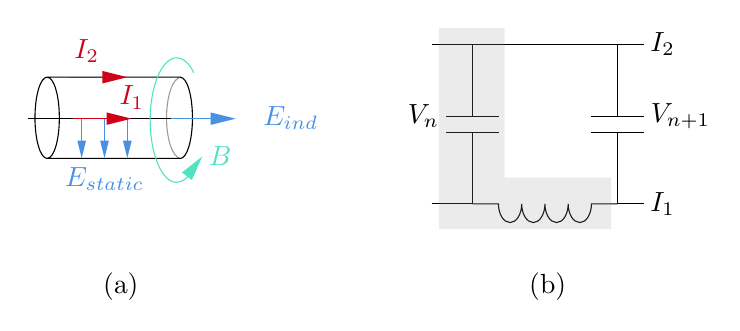
\begin{tikzpicture}[x=0.75pt,y=0.75pt,yscale=-1,xscale=1]
    %uncomment if require: \path (0,300); %set diagram left start at 0, and has height of 300
    
    %Shape: Arc [id:dp5331133978803468] 
    \draw  [draw opacity=0] (179.13,164.25) .. controls (175.44,163.61) and (172.51,155.1) .. (172.51,144.7) .. controls (172.51,134.08) and (175.56,125.44) .. (179.36,125.12) -- (179.58,144.7) -- cycle ; \draw  [color={rgb, 255:red, 155; green, 155; blue, 155 }  ,draw opacity=1 ] (179.13,164.25) .. controls (175.44,163.61) and (172.51,155.1) .. (172.51,144.7) .. controls (172.51,134.08) and (175.56,125.44) .. (179.36,125.12) ;  
    %Straight Lines [id:da12247143299984486] 
    \draw    (300.46,109.33) -- (319.83,109.33) ;
    %Straight Lines [id:da6109342480428939] 
    \draw    (319.83,109.33) -- (389.83,109.33) ;
    %Shape: Capacitor [id:dp8125842692023104] 
    \draw   (319.83,109.33) -- (319.83,143.9) (332.58,151.58) -- (307.08,151.58) (332.58,143.9) -- (307.08,143.9) (319.83,151.58) -- (319.83,186.15) ;
    %Shape: Capacitor [id:dp3820330659104405] 
    \draw   (389.83,109.33) -- (389.83,143.9) (402.58,151.58) -- (377.08,151.58) (402.58,143.9) -- (377.08,143.9) (389.83,151.58) -- (389.83,186.15) ;
    %Shape: Inductor (Air Core) [id:dp21252438201509394] 
    \draw   (389.83,186.15) -- (377.23,186.15) .. controls (377.23,191.11) and (374.72,195.15) .. (371.63,195.15) .. controls (368.54,195.15) and (366.03,191.11) .. (366.03,186.15) .. controls (366.03,191.11) and (363.52,195.15) .. (360.43,195.15) .. controls (357.34,195.15) and (354.83,191.11) .. (354.83,186.15) .. controls (354.83,191.11) and (352.32,195.15) .. (349.23,195.15) .. controls (346.14,195.15) and (343.63,191.11) .. (343.63,186.15) .. controls (343.63,191.11) and (341.12,195.15) .. (338.03,195.15) .. controls (334.94,195.15) and (332.43,191.11) .. (332.43,186.15) -- (319.83,186.15) ;
    %Straight Lines [id:da21200291272484972] 
    \draw    (389.83,109.33) -- (402.33,109.33) ;
    %Straight Lines [id:da041781966587811414] 
    \draw    (300.21,186.15) -- (319.83,186.15) ;
    %Straight Lines [id:da4699416797302651] 
    \draw    (389.83,186.15) -- (402.33,186.15) ;
    %Shape: Can [id:dp23647903681372484] 
    \draw   (115,125.1) -- (179.13,125.1) .. controls (182.37,125.1) and (185,133.87) .. (185,144.68) .. controls (185,155.49) and (182.37,164.25) .. (179.13,164.25) -- (115,164.25) .. controls (111.75,164.25) and (109.13,155.49) .. (109.13,144.68) .. controls (109.13,133.87) and (111.75,125.1) .. (115,125.1) .. controls (118.24,125.1) and (120.87,133.87) .. (120.87,144.68) .. controls (120.87,155.49) and (118.24,164.25) .. (115,164.25) ;
    %Straight Lines [id:da8686341750411] 
    \draw    (105.88,145.1) -- (196,145.1) ;
    %Straight Lines [id:da6849184867595193] 
    \draw [color={rgb, 255:red, 74; green, 144; blue, 226 }  ,draw opacity=1 ]   (131.63,145.1) -- (131.63,162.1) ;
    \draw [shift={(131.63,164.1)}, rotate = 270] [fill={rgb, 255:red, 74; green, 144; blue, 226 }  ,fill opacity=1 ][line width=0.08]  [draw opacity=0] (8.4,-2.1) -- (0,0) -- (8.4,2.1) -- cycle    ;
    %Shape: Arc [id:dp3677584369492668] 
    \draw  [draw opacity=0] (185.67,168.56) .. controls (183.44,173.05) and (180.54,175.77) .. (177.38,175.77) .. controls (170.33,175.77) and (164.63,162.34) .. (164.63,145.77) .. controls (164.63,129.2) and (170.33,115.77) .. (177.38,115.77) .. controls (180.54,115.77) and (183.44,118.49) .. (185.67,122.98) -- (177.38,145.77) -- cycle ; \draw  [color={rgb, 255:red, 80; green, 227; blue, 194 }  ,draw opacity=1 ] (185.67,168.56) .. controls (183.44,173.05) and (180.54,175.77) .. (177.38,175.77) .. controls (170.33,175.77) and (164.63,162.34) .. (164.63,145.77) .. controls (164.63,129.2) and (170.33,115.77) .. (177.38,115.77) .. controls (180.54,115.77) and (183.44,118.49) .. (185.67,122.98) ;  
    %Straight Lines [id:da5720848890832353] 
    \draw [color={rgb, 255:red, 80; green, 227; blue, 194 }  ,draw opacity=1 ]   (185.67,168.56) -- (188.49,164.92) ;
    \draw [shift={(189.71,163.34)}, rotate = 127.8] [fill={rgb, 255:red, 80; green, 227; blue, 194 }  ,fill opacity=1 ][line width=0.08]  [draw opacity=0] (12,-3) -- (0,0) -- (12,3) -- cycle    ;
    %Straight Lines [id:da08490537832946576] 
    \draw [color={rgb, 255:red, 74; green, 144; blue, 226 }  ,draw opacity=1 ]   (174.88,145.1) -- (203.75,145.1) ;
    \draw [shift={(205.75,145.1)}, rotate = 180] [fill={rgb, 255:red, 74; green, 144; blue, 226 }  ,fill opacity=1 ][line width=0.08]  [draw opacity=0] (12,-3) -- (0,0) -- (12,3) -- cycle    ;
    %Straight Lines [id:da5107008145824161] 
    \draw [color={rgb, 255:red, 74; green, 144; blue, 226 }  ,draw opacity=1 ]   (142.63,145.1) -- (142.63,162.1) ;
    \draw [shift={(142.63,164.1)}, rotate = 270] [fill={rgb, 255:red, 74; green, 144; blue, 226 }  ,fill opacity=1 ][line width=0.08]  [draw opacity=0] (8.4,-2.1) -- (0,0) -- (8.4,2.1) -- cycle    ;
    %Straight Lines [id:da5804823414578775] 
    \draw [color={rgb, 255:red, 74; green, 144; blue, 226 }  ,draw opacity=1 ]   (153.63,145.1) -- (153.63,162.1) ;
    \draw [shift={(153.63,164.1)}, rotate = 270] [fill={rgb, 255:red, 74; green, 144; blue, 226 }  ,fill opacity=1 ][line width=0.08]  [draw opacity=0] (8.4,-2.1) -- (0,0) -- (8.4,2.1) -- cycle    ;
    %Straight Lines [id:da2696125138845171] 
    \draw [color={rgb, 255:red, 208; green, 2; blue, 27 }  ,draw opacity=1 ][fill={rgb, 255:red, 208; green, 2; blue, 27 }  ,fill opacity=1 ]   (127.38,145.1) -- (153.63,145.1) ;
    \draw [shift={(155.63,145.1)}, rotate = 180] [fill={rgb, 255:red, 208; green, 2; blue, 27 }  ,fill opacity=1 ][line width=0.08]  [draw opacity=0] (12,-3) -- (0,0) -- (12,3) -- cycle    ;
    %Straight Lines [id:da2708166657474578] 
    \draw [color={rgb, 255:red, 208; green, 2; blue, 27 }  ,draw opacity=1 ][fill={rgb, 255:red, 208; green, 2; blue, 27 }  ,fill opacity=1 ]   (125.38,125.1) -- (151.63,125.1) ;
    \draw [shift={(153.63,125.1)}, rotate = 180] [fill={rgb, 255:red, 208; green, 2; blue, 27 }  ,fill opacity=1 ][line width=0.08]  [draw opacity=0] (12,-3) -- (0,0) -- (12,3) -- cycle    ;
    %Shape: Path Data [id:dp48367091522979666] 
    \draw  [draw opacity=0][fill={rgb, 255:red, 155; green, 155; blue, 155 }  ,fill opacity=0.2 ] (335.46,101.52) -- (335.46,173.44) -- (386.71,173.44) -- (386.71,198.27) -- (303.71,198.27) -- (303.71,101.52) -- (335.46,101.52) -- cycle ;
    
    % Text Node
    \draw (305.08,143.9) node [anchor=east] [inner sep=0.75pt]    {$V_{n}$};
    % Text Node
    \draw (404.58,143.9) node [anchor=west] [inner sep=0.75pt]    {$V_{n+1}$};
    % Text Node
    \draw (148.63,134.94) node [anchor=west] [inner sep=0.75pt]  [color={rgb, 255:red, 208; green, 2; blue, 27 }  ,opacity=1 ]  {$I_{1}$};
    % Text Node
    \draw (142.63,167.5) node [anchor=north] [inner sep=0.75pt]  [color={rgb, 255:red, 74; green, 144; blue, 226 }  ,opacity=1 ]  {$E_{\text{static}}$};
    % Text Node
    \draw (191.71,163.34) node [anchor=west] [inner sep=0.75pt]  [color={rgb, 255:red, 74; green, 144; blue, 226 }  ,opacity=1 ]  {$\textcolor[rgb]{0.31,0.89,0.76}{B}$};
    % Text Node
    \draw (217.88,144.68) node [anchor=west] [inner sep=0.75pt]  [color={rgb, 255:red, 74; green, 144; blue, 226 }  ,opacity=1 ]  {$E_{\text{ind}}$};
    % Text Node
    \draw (140.67,218.19) node [anchor=north west][inner sep=0.75pt]   [align=left] {(a)};
    % Text Node
    \draw (346,218.19) node [anchor=north west][inner sep=0.75pt]   [align=left] {(b)};
    % Text Node
    \draw (126.88,112.44) node [anchor=west] [inner sep=0.75pt]  [color={rgb, 255:red, 208; green, 2; blue, 27 }  ,opacity=1 ]  {$I_{2}$};
    % Text Node
    \draw (404.33,109.33) node [anchor=west] [inner sep=0.75pt]    {$I_{2}$};
    % Text Node
    \draw (404.33,186.15) node [anchor=west] [inner sep=0.75pt]    {$I_{1}$};
    
    
    \end{tikzpicture}
    